\section{Connectivité dans les Graphes : Concepts et Applications}

La connectivité est un pilier central de la théorie des graphes, qui s'intéresse aux diverses manières dont les éléments d'un graphe peuvent être reliés ou séparés. Cette section approfondit les notions de connectivité, en définissant des termes essentiels et en présentant le théorème de Menger, une pierre angulaire dans l'étude des graphes.

\begin{figure}[H]
    \centering
    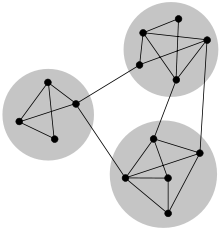
\includegraphics[width=0.3 \textwidth]{Assets/connectivite.png}
    \caption{Connectivité (théorie des graphes)}
    \label{fig:Connectivité (théorie des graphes)}
\end{figure}


\subsection{Graphe Connecté}
Un graphe non orienté est dit connecté si, pour toute paire de sommets, il existe un chemin les reliant. Cette propriété assure qu'aucun sommet n'est isolé, permettant une traversée intégrale du graphe.

\begin{figure}[H]
    \centering
    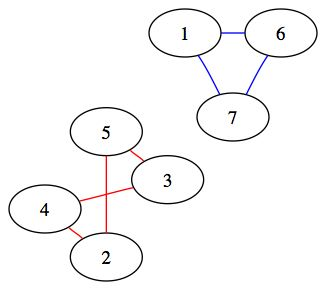
\includegraphics[width=0.3 \textwidth]{Assets/graphe connecte.jpg}
    \caption{Graphe Connecté}
    \label{fig:Graphe Connecté}
\end{figure}

\subsection{Graphe Fortement Connecté}
Un graphe orienté est fortement connecté si, pour toute paire de sommets \( u \) et \( v \), il existe un chemin de \( u \) à \( v \) et un chemin de \( v \) à \( u \). Cette forte connectivité indique une interdépendance complète entre les sommets, permettant une circulation sans restriction dans toutes les directions.

\begin{figure}[H]
    \centering
    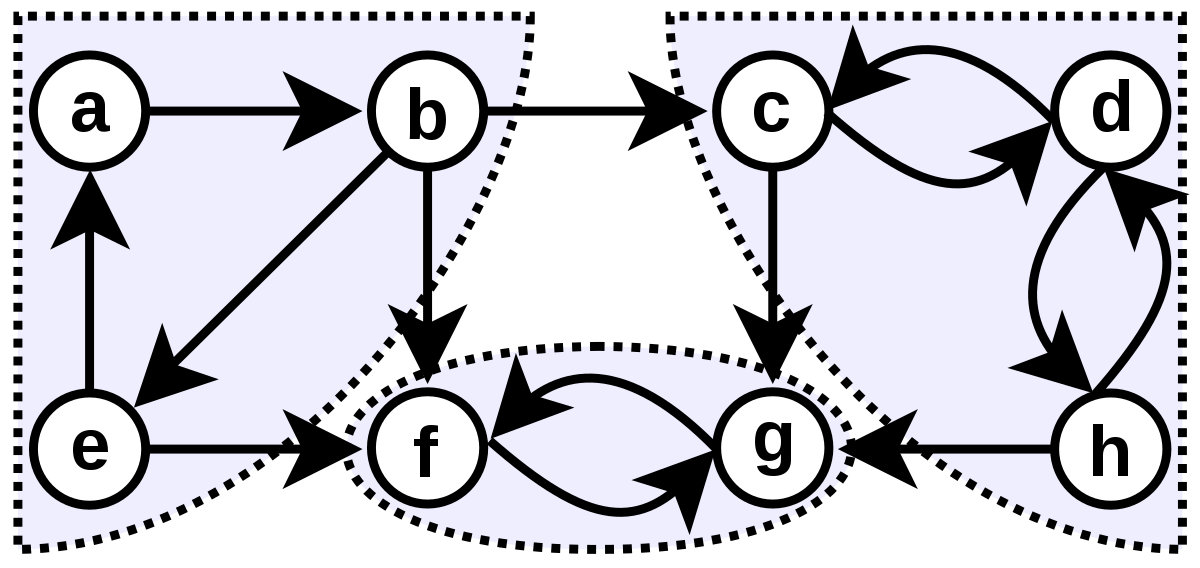
\includegraphics[width=0.3 \textwidth]{Assets/graphe fortement connecte.png}
    \caption{Graphe Fortement Connecté}
    \label{fig:Graphe Fortement Connecté}
\end{figure}

\subsection{Graphe Faiblement Connecté}
Un graphe orienté est faiblement connecté si, en ignorant la direction des arêtes, le graphe devient connecté. Cela signifie que même sans considérer l'orientation, il est possible de relier tous les sommets entre eux, témoignant d'une certaine résilience de la structure du graphe.



\newpage


\subsection{Connectivité de Sommet et d'Arête}
La connectivité de sommet, \( \kappa(G) \), est le nombre minimal de sommets dont la suppression (avec leurs arêtes incidentes) fragmente le graphe en composantes non connectées. La connectivité d'arête, \( \lambda(G) \), est le nombre minimal d'arêtes dont la suppression déconnecte le graphe. Ces deux mesures évaluent la vulnérabilité d'un graphe face aux perturbations.

\subsection{Théorème de Menger}
Le théorème de Menger fournit un lien fondamental entre la connectivité de sommet, la connectivité d'arête, et l'existence de chemins indépendants. Il stipule que pour deux sommets non adjacents \( u \) et \( v \), le nombre minimal de sommets à supprimer pour séparer \( u \) de \( v \) est égal au nombre maximal de chemins indépendants reliant \( u \) à \( v \). Ce théorème est essentiel pour comprendre la robustesse et la redondance des chemins dans un réseau.
\begin{figure}[H]
    \centering
    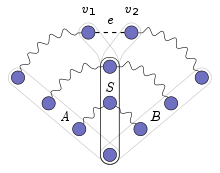
\includegraphics[width=0.4 \textwidth]{Assets/menger.png}
    \caption{Théorème de Menger}
    \label{fig:Théorème de Menger}
\end{figure}
